\section{Introduction}
\label{Chapter:Introduction}
{
    \IEEEPARstart{T}{he} art of Islamic calligraphy has a history that dates back to the seventh century \cite{bib01, bib02}. It has witnessed many evolutionary stages \cite{bib02, bib03} and has been used by artists speaking several different languages \cite{bib04} and sharing uncommon biographies \cite{bib05,bib06,bib07,bib08}. Unfortunately though, the industrial age and the advent of technology has not spared this beautiful art from its subsuming tide, with traditional calligraphy struggling to keep up with digitization and dwindling community support. The very existence of Islamic calligraphy now faces a serious threat. Public buildings and infrastructure that once used to be a showcase for the most laudable artists of the time have turned into museums; awaiting to be wiped away slowly with each round of the monsoon and every splash of the ocean’s waves. One such site is shown in Figure \ref{Fig:BegumShahi}.

    \begin{figure}[!t]
        \centering
        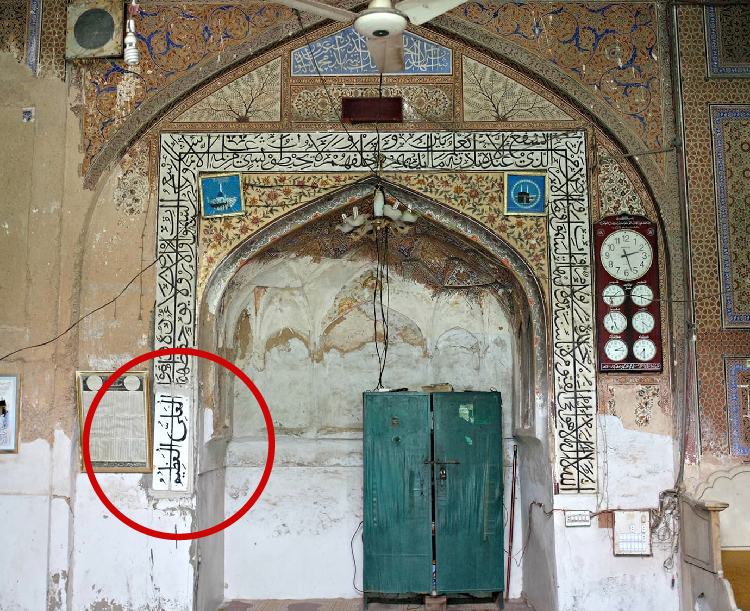
\includegraphics[width=2.5in]{../Images/BegumShahi.jpg}
        \caption{A photo of a wall inside Mariyam Zamani Mosque (also known as Begum Shahi Masjid) Lahore. Some of the calligraphy has been reconstructed (highlighted in red) using conventional techniques and can easily be recognised because it looks different than the rest.}
        \label{Fig:BegumShahi}
    \end{figure}
%
%
%    \begin{figure}
%      \centering
%      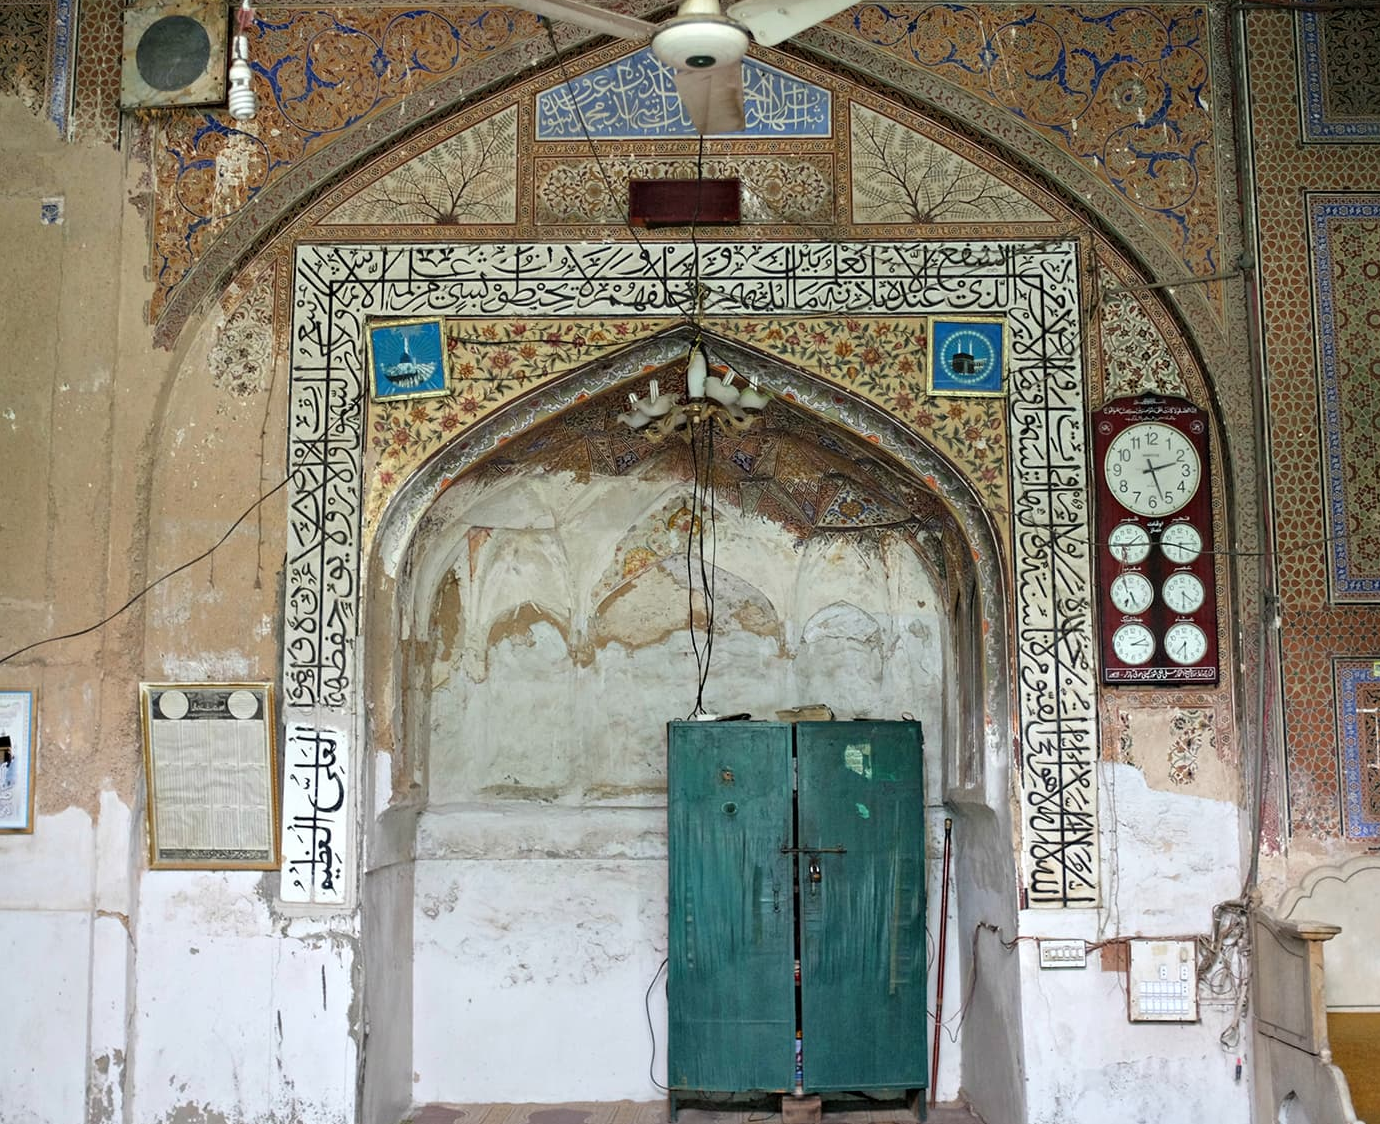
\includegraphics[width=0.9\textwidth]{../Images/BegumShahi.pdf}
%      \caption{A photo of a wall inside Mariyam Zamani Mosque (also known as Begum Shahi Masjid) Lahore. Some of the calligraphy has been reconstructed (highlighted in red) using conventional techniques and can easily be recognised because it looks different than the rest.
%      } \label{Fig:BegumShahi}
%    \end{figure}


    Potentially, we can use robotic dexterity to help us in this domain. Industrial robots have already been used in the field to perform unorthodox tasks such as \cite{bib09, bib10,bib11,bib12} and they can surely uplift this art as well. At the very least, they can be employed in restoration and replication of existing calligraphic work \cite{bib13}. In other words, they can be used as printers, or rather one may say, ``painters'' that give an extra hand to the calligraphers to open up new dimensions of art work that can not only revamp existing calligraphy sites but also create new ones.

    Mechanized robotic drawing of the Islamic calligraphy scripts requires not just the ink-mark information but also the information about the tool movement \cite{bib03}. Compared to industrial color printers that mostly print on flat surfaces, or rolled surfaces at best, using a flexible broad edge brush to draw on possibly uneven curved surfaces situated in narrow spaces, makes the job relatively more complex. This complexity arises because in this realm, in addition to normal tool movement information, a robot needs to take special care about the orientation of a flexible tool and its surface facing force as well.

    Since an industrial robotic arm can accurately maneuver paths in three dimensional space with controlled speed and downward force, the residual problem can be mainly divided in two parts. First, discover a method that can not only digitize existing Islamic calligraphy specimens but can also allow modifying and creating new ones. Second, discovering a method to extract machine data from graphical data.

    This research proposes one solution to answer both of these questions: unifying graphical data with machine data. Conventionally, the kind of data used by the computer to render and print graphics on the screen or on paper fundamentally differs from the data needed by a machine [cite] that uses a mechanical end-effector to produce output. We propose a rather simple innovation in the conventional bezier splines which enables them to mimic the ink-mark of broad-edge tools and can directly generate machine movement data. We name them ``Rotating or Twisting Bezier Spline Curves'', or simply, ``Twisting Bezier Splines''.

    There are still some challenges which need consideration even with a twisting bezier spline. The inkmark in most islamic calligraphy scripts is usually a result of multiple closely located tool strokes [cite] that form up words using overlapping letters. Furthermore, as a result of spin of a broad-edge tool, the width of the strokes continuously varies. No computer algorithm currently exists that can accurately determine the pitch lines of these islamic calligraphy strokes because of the aforementioned complexities. Twisting bezier splines can intrinsically extract this pitch line during the tracing process.

    The article is divided in $5$ sections. After the introduction, we briefly highlight the related complexities involved in writing islamic scripts in Chapter \ref{Chapter:ScriptComplexities}. Chapter \ref{Chapter:SplineModelling} then presents the working principle and mathematical model of the twisting bezier splines. In section \ref{Chapter:Performance} we discuss some performance metric and discuss the tests performed to gauge the performance of the twisting bezier splines. Section \ref{Chapter:Simulation} discusses the simulation of machine data produced using twisting bezier splines of a robotic manipulator in order to validate the results. We finally conclude in Section \ref{Chapter:Conclusion}. The software tools used in this research, the software user manuals, video tutorials and the source codes can be viewed on the project GitHub repo\cite{bib20}.
}
\section{Challenges Involved in Digitizing Islamic Calligraphy}
\label{Chapter:ScriptComplexities}
{
    \noindent Islamic calligraphy is mostly performed in scripts that are used to write Arabic, Urdu, Persian and similar languages. These scripts share some common traits that make their digitization a challenge.

    \begin{itemize}
    \item Most of the times, the individual letters have to overlap with each other to form a complete word. See Figure \ref{Fig:UrduScriptBreakDown}(a), (b) and (c). This makes it difficult to break down words into individual letters.
    \item Most of the letters can appear in multiple forms depending upon its position in the word as well as the artist's discretion. Figure \ref{Fig:UrduScriptBreakDown}(d) shows a compound word that uses letters in multiple shapes.
    \item Most of the times, a single stroke of pen is used to write major portions of words that include multiple overlapping letters.
    \item Many a times, parts of words and letters that seem to be drawn using a single stroke are actually drawn using multiple strokes and are only made to look like a continuous stroke. See Figure \ref{Fig:Nastaleeq}(c) and \ref{Fig:Thuluth}(c) which shows overlapping regions of multiple strokes that overall have the look of a single stroke.
    \end{itemize}

    \begin{figure}[!t]
        \centering
        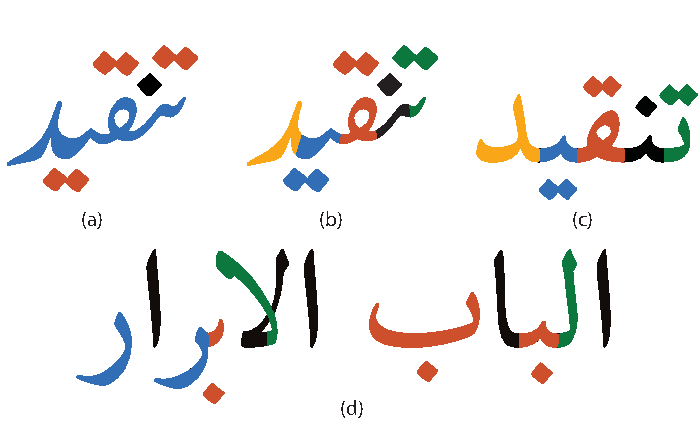
\includegraphics[width=2.5in]{../Images/Nuqtah.pdf}
        \caption{Words written in Nastaleeq and Naqsh styles. (a), (b) and (c) show three different representations of a single word. In (a) the word is written in Nastaleeq style containing parts that appear as a single continuous stroke of tool (highlighted in distinct colors). (b) and (c) show the same word in Nastaleeq and Naskh style respectively and each letter is highlighted in different colors. (d) A compound word written in Naskh style that uses some letters multiple times but in different shapes. All occurrences of a single letter are painted in a distinct color.}
        \label{Fig:UrduScriptBreakDown}
    \end{figure}

}
